\newpage
\section{BUSINESS MODEL} \label{businessmodel}

As we described in Section \ref{landscape}, the online digital content market can be grouped in two major business models, namely Maker and Exchange Platforms. Both solution have a centralized nature and impose great restrictions to Creators and Buyers.

BlockLicense introduces a new business model that puts Creators and Buyers at the forefront by removing all restrictions imposed by Maker and Exchange Platforms and by  providing tools that simplify the licensing process and allow a wide range of licensing scenarios. Payment processing and routing as well as proof-of-ownership is automated with Ethereum smart contracts.

Multiple channels of distribution are provided including a Web Platform, website embedded shops \& offline distribution of files. All transactions and payouts within BlockLicense are instant while both creators and buyers are free of subscription or hidden costs. A flat 2\% fee is imposed in all transactions to cover BlockLicense costs and allow a continuous and organic expansion of the ecosystem.

\begin{figure}[h]
\centering
\begin{minipage}{.45\textwidth}
  \centering
  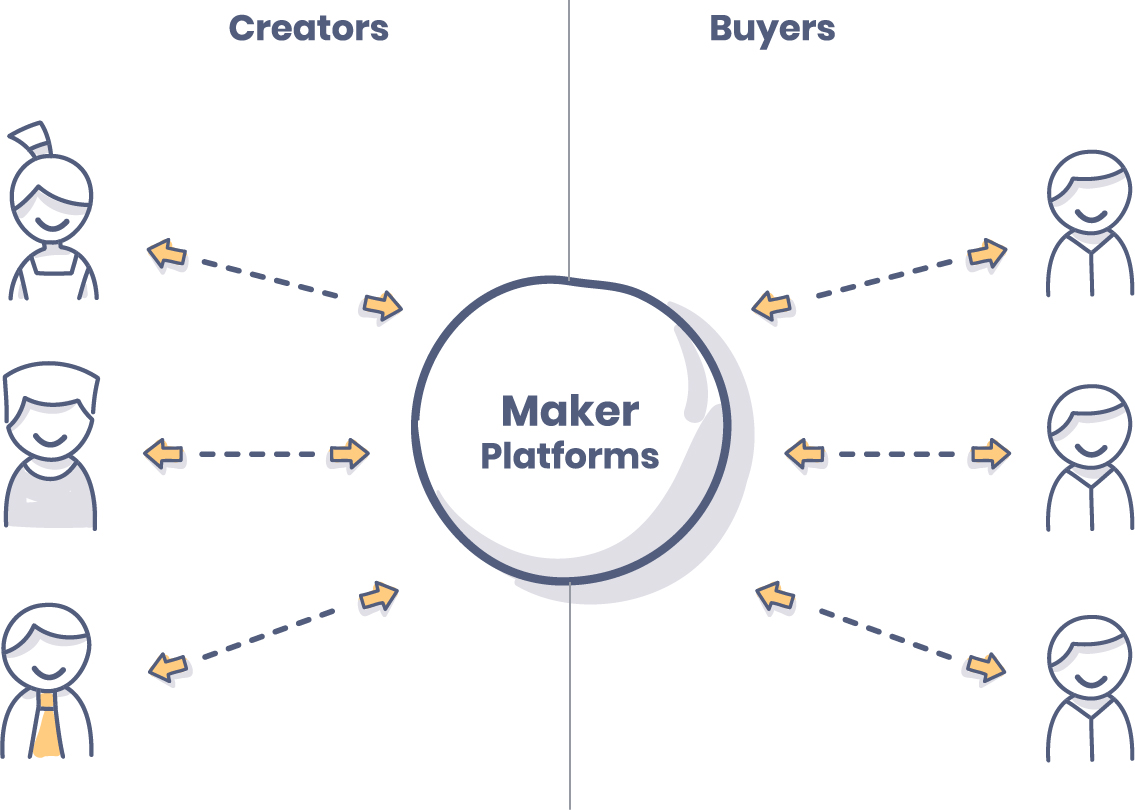
\includegraphics[width=.8\linewidth]{./figures/fig9.jpg}
  \caption{Maker Platforms.}
  \label{fig:maker}
\end{minipage}
\begin{minipage}{.45\textwidth}
  \centering
  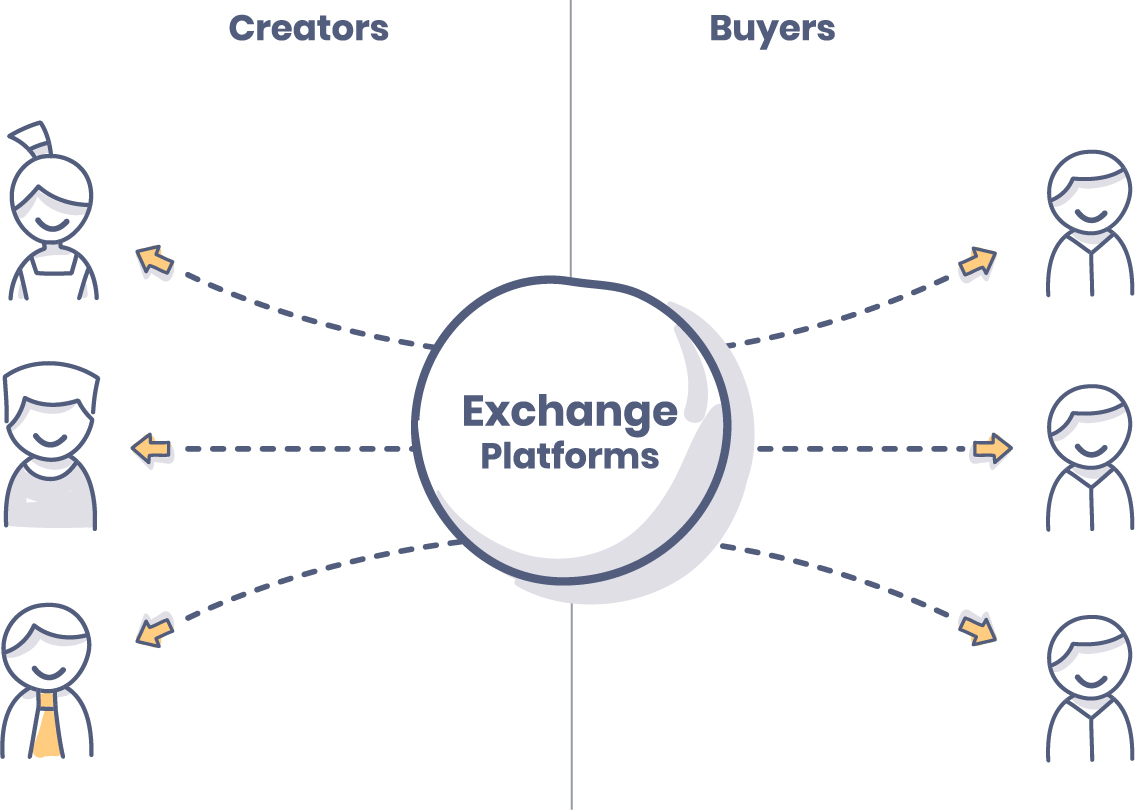
\includegraphics[width=.8\linewidth]{./figures/fig10.jpg}
  \caption{Exchange Platforms.}
  \label{fig:exchange}
\end{minipage}%
\end{figure}
 
\subsection{Sustainability}

A solid and growing community is paramount to the BlockLicense success. Like any other innovation, a certain time will be needed before it penetrates the market.  The adoption period, for new technologies, looks like an ‘S’ curve \cite{pierre}, as shown in Figure \ref{fig:scurve}, where customer segmentation is spread among five main categories: innovators, early adopters, early majority, late majority and laggards.

Once the crowdfunding campaign starts 
It is expected that on pre-, on and post-launch period, BlockLicense will gain market momentum, forming a noteworthy community of innovators and early adopters that will later expand to include early and late majority members. 

With an aim of achieving a 3\% of market share by the sixth year of  BlockLicense's operation, it is fundamental that  continuous marketing activities take place that focus on bringing additional value to the Blocklicense community. Activities may include incentives for both creators and buyers to use the ecosystem such as, \textit{bonus schemes} and \textit{ambassador programs} to name a few. Yet alone, marketing activities and incentives are not capable of growing or even maintaining the community. BlockLicense aims to constantly improve and expand the ecosystem by looking at the community needs.

\begin{figure}[h]
\centering
\begin{minipage}{1\textwidth}
  \centering
  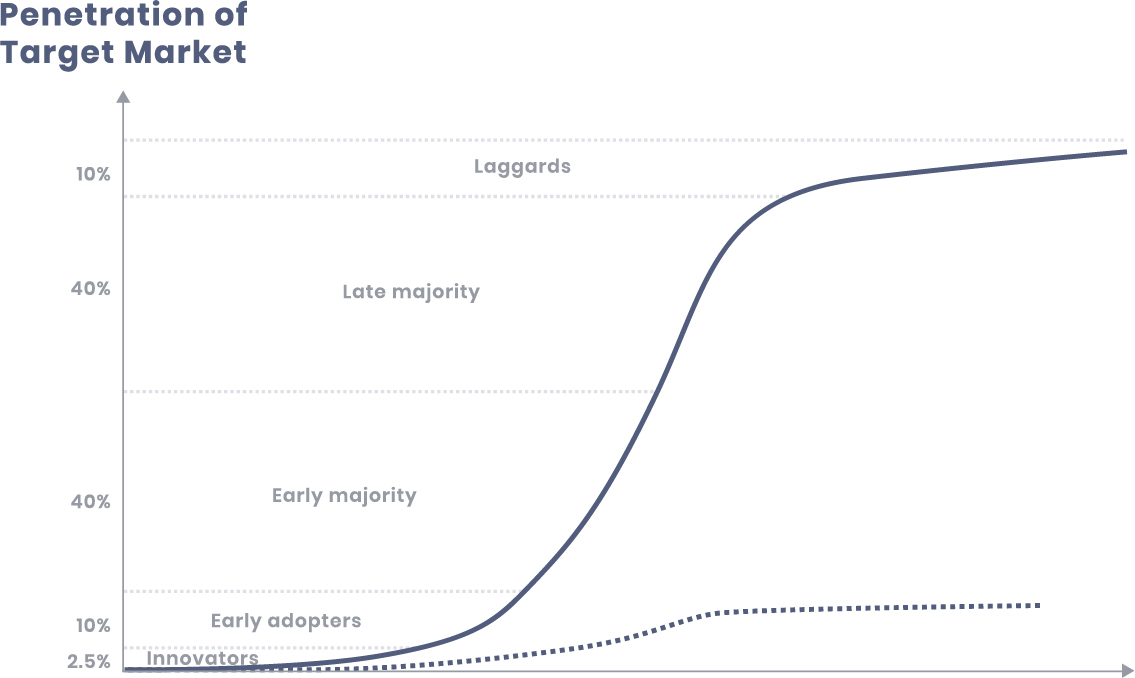
\includegraphics[width=.8\linewidth]{./figures/fig11.jpg}
  \caption{Market Penetration.}
  \label{fig:scurve}
\end{minipage}
\end{figure}